\SetKwRepeat{Struct}{struct \{}{\}}%
\newcommand{\Array}{\KwSty{Array}}
\newcommand{\Integer}{\KwSty{Integer}}

\chapter{Task-Based, Parallel and Distributed Sparse Linear Algebra Applications}
\graphicspath{{chapters/exp_sparse/}}

The sparse matrix vector product with several matrix storage format and matrix distribution across the computing resources is basic algorithm considered in this chapter.
The sparse operation $A(Ax+x)$ is also considered as it uses two times the sparse matrix vector product.


\section{Task-Based Methods for Parallel and Distributed Algorithms}
The sparse matrix vector product is executed in a distributed and parallel environment which means that computations can be run in parallel and data may not be accessed directly since they can be stored on a different resource than where they are needed.
The data can be moved through the network but it can be costly especially in very large networks.
The goal is to implement a parallel, distributed and task based sparse matrix vector product taking advantage of this set up while getting the best execution time and reducing the communications.
In the sparse matrix vector product case, the distributed and parallel algorithms (both regular and task based) depends on the storage formats used and the distribution of the sparse matrix on the distributed resources.
There is several way of distributing the matrix : either by splitting the columns or the rows.
A combination of the two previous way of distribution, the block distribution is also considered here.
They are the main way of distributing a matrix although other ways exist like a cyclic distribution where the consecutive values are put alternatively on a distributed resource.


\subsection{Data Distribution \label{sec:sla:data_distribution}}

We consider three ways of distributing the data : a distribution by rows, by columns and by blocks.
The distribution by rows and by columns are special cases of the distribution by blocks where the is only distribution across one row for the distribution by columns and where the is only distribution across one column for the distribution by rows.


\begin{figure}[h]
	\centering
	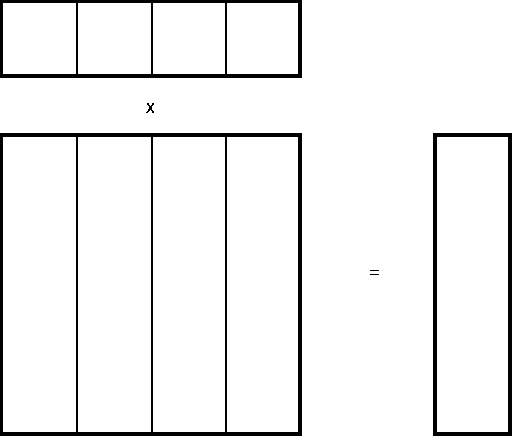
\includegraphics[width=.5\textwidth]{pmv_c}
	\caption{Distribution of the matrix by columns \label{fig:sparse:pmv_c}}
\end{figure}

The distribution by columns consists in splitting the rows and keeping the values of the same column in the same computing resource.
The input vector can also be split since only the rows of the vector corresponding to the columns stored in a computing resource are necessary for the matrix vector product.
The Figure \ref{fig:sparse:pmv_c} shows a matrix distributed by rows to make a matrix product vector as well as the necessary input vector and the result vector.
The result vector has the same size as the number of rows in the sub-matrices.
In this case, it corresponds to the full matrix number of rows.
However, each computing resource contains a part of the global solution of the matrix vector product.
To obtain the global result, all the distributed results have to be summed.


\begin{figure}[h]
	\centering
	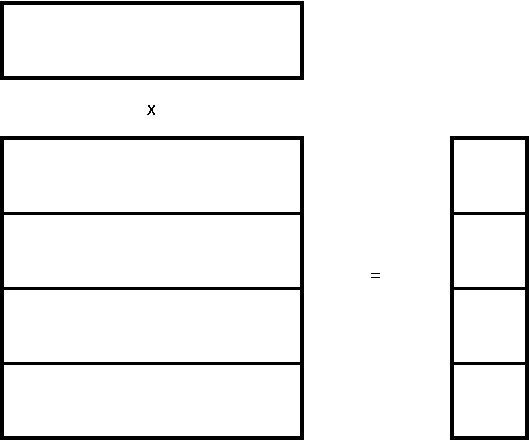
\includegraphics[width=.5\textwidth]{pmv_r}
	\caption{Distribution of the matrix by rows\label{fig:sparse:pmv_r}}
\end{figure}

The distribution by rows consists in splitting the columns and keeping the values of the same row in the same computing resource.
In this case, the input vector cannot be split since a complete row of the matrix may be stored in each computing resource.
In the sparse case, the rows may not be complete on each process but it can not be known in advance.
The input vector will be duplicated in each computing resource.
The result vector has the same size as the number of rows in the sub-matrices.
Here, it corresponds to the number of rows in each corresponding sub-matrices.
However, each computing resource contains a sub-vector.
To obtain the global result, all the distributed results have to be gathered (which means that the global vector has just to be reconstructed without any computations).


\begin{figure}[h]
	\centering
	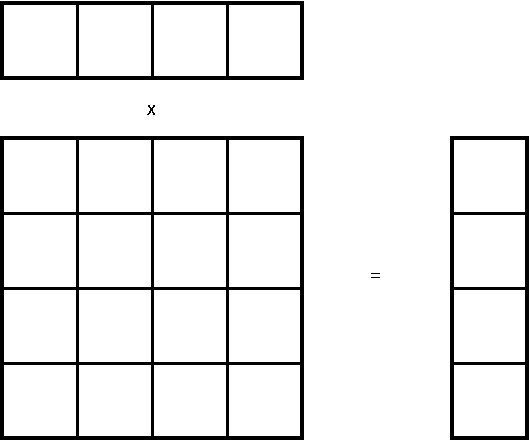
\includegraphics[width=.5\textwidth]{pmv_2D}
	\caption{Distribution of the matrix by rows and columns\label{fig:sparse:pmv_2D}}
\end{figure}

The block distribution consists in both a distribution by rows and distribution by columns.
The matrix in split in a 2D grid way.
The $Nx \times Ny$ matrix is split in $Ngx \times Ngy$ sub-matrices.
In this case, the input vector is split across the columns of the matrix and the sub-vectors are duplicated on the sub-rows of the same column.
The Figure \ref{fig:sparse:pmv_r} shows a matrix distributed by blocks to perform a matrix product vector as well as the necessary input vector and the result vector with $Ngx = 4$ and $Ngy = 4$.
The result vector has the same size as the number of rows in the sub-matrices of the corresponding row.
However, each computing resource contains a part of a sub-vector.
To obtain the global result, all the distributed results of the same row have to be reduced then each rows have to be gathered if the full result vector is needed in one place.

The data distribution determines which part of the global matrix will be stored on a given computing resource.
The Section \ref{sec:sla:task_definition} points out how these data will be used to perform the matrix vector product.

\subsection{Tasks Definition \label{sec:sla:task_definition}}

In this section, we consider that the matrix is divided according to one of the distribution described previously (except for the COO storage format).
Each sub-matrix will be used as input of the matrix vector product tasks defined in the following algorithms.
We will define data structures to store the matrices and use them in the tasks.
Finally, the algorithms for the tasks will be designed.


\begin{algorithm}[h]
	\DontPrintSemicolon
	\SetAlgoVlined
	\caption{COO format data structure and matrix vector product\label{alg:sparse:spmv_coo}}
	\SetKwProg{Fn}{Task}{}{end}

	\Struct{MatrixCOO}{
		\Array{} row, col, val\;
	}
	\;
	\Fn{spmv\_coo()}{
		\KwData{m : MatrixCOO, v : Array}
		\KwResult{r : Array}
		\For{i \KwFrom 0 \KwTo m.val.size() - 1}{
			r[m.row[i]] += m.val[i] * v[m.col[i]]\;
		}
	}
\end{algorithm}

Algorithm \ref{alg:sparse:spmv_coo} defines a data structure to store the sub-matrices stored in the COO format.
It also shows the algorithm to make a matrix vector product on the sub-matrix given the proper input vector.
The data structure contains the three arrays necessary to store the matrix in the COO storage format.
In this implementation of the matrix vector product with the COO format, the sub-matrix does not have to be sorted e.g. this implementation does not expect the coordinates of the values of the matrix to be in a given range.
Therefore, this implementation can process any value in any position in any sub-matrix (which is not the case with the other storage formats).
However, we cannot deduce the range of position in the full input vector which will be effectively used in the task as well as the range of position for the output vector since there is no restrictions on the range of coordinates of the values in the matrix.
Thus, this task also expect the full vector as input for the tasks (independently of the data distribution described) and output a full vector.

It can allow a better load balancing at the cost of a full vector in input and output which will change how the output vector will be processed to construct the full output vector.
This will be discussed in Section \ref{sec:sla:task_based_parallel_algorithms}.


\begin{algorithm}[h]
	\DontPrintSemicolon
	\SetAlgoVlined
	\caption{SCOO format data structure and matrix vector product\label{alg:sparse:spmv_scoo}}
	\SetKwProg{Fn}{Task}{}{end}

	\Struct{MatrixSCOO}{
		\Array{} row, col, val\;
		\Integer{} fr, fc\;
	}
	\;
	\Fn{spmv\_scoo()}{
		\KwData{m : MatrixCOO, v : Array}
		\KwResult{r : Array}
		\For{i \KwFrom 0 \KwTo m.val.size() - 1}{
			r[m.row[i] - m.fr] += m.val[i] * v[m.col[i] - m.fc]\;
		}
	}
\end{algorithm}

Algorithm \ref{alg:sparse:spmv_scoo} defines a data structure to store the sub-matrices stored in the SCOO format in which we expect a given range of coordinates for the values contrary to the COO format.
It also shows the algorithm to make a matrix vector product on the sub-matrix given the proper input vector.
The data structure contains the three arrays necessary to store the matrix in the SCOO storage format as well as useful informations about the position of the sub-matrix in the global matrix.
These informations are the first row (\textit{fr}) and the first column (\textit{fc}) possibles in the sub-matrix (It may not correspond to the actual values stored in the sub-matrix since it corresponds to the lower boundaries of the possible coordinates in the sub-matrix for the algorithm to work properly).
The algorithm for the SCOO storage format is similar to the algorithm for COO whereas the supplementary informations are used in the algorithm to properly position the output vector.
In this case, the range of position for the input and output vectors can be computed since the range of coordinates for the values in the SCOO storage format are restricted to the data distributions discussed in Section \ref{sec:sla:data_distribution}.
Therefore, depending of the data distribution, the input and output vector shapes change.

In this case, the construction of the full output vector will depend on the division of the matrix as specified in Section \ref{sec:sla:data_distribution}.
This will be detailed further in Section \ref{sec:sla:task_based_parallel_algorithms}.


\begin{algorithm}[h]
	\DontPrintSemicolon
	\SetAlgoVlined
	\caption{CSR format data structure and matrix vector product\label{alg:sparse:spmv_csr}}
	\SetKwProg{Fn}{Task}{}{end}

	\Struct{MatrixCSR}{
		\Array{} idx, col, val\;
		\Integer{} fc\;
	}
	\;
	\Fn{spmv\_csr()}{
		\KwData{m : MatrixCSR, v : Array}
		\KwResult{r : Array}
		\For{i \KwFrom 0 \KwTo m.idx.size() - 1}{
			\For{j \KwFrom m.idx[i] \KwTo m.idx[i+1] - 1}{
				r[i] += m.val[j] * v[m.col[j] - m.fc]\;
			}
		}
	}
\end{algorithm}

Algorithm \ref{alg:sparse:spmv_csr} defines a data structure to store the sub-matrices stored in the CSR format in which we expect a given range of coordinates for the values.
It also shows the algorithm to make a matrix vector product on the sub-matrix given the proper input vector.
The data structure contains the three arrays necessary to store the matrix in the CSR storage format as well as useful informations about the position of the sub-matrix in the global matrix.
These informations are the first column (\textit{fc}) possibles in the sub-matrix.
As for the COO storage format, the ranges of position for the input and output vectors can be computed.


\begin{algorithm}[h]
	\DontPrintSemicolon
	\SetAlgoVlined
	\caption{ELL format data structure and matrix vector product\label{alg:sparse:spmv_ell}}
	\SetKwProg{Fn}{Task}{}{end}

	\Struct{MatrixELL}{
		\Array{} col, val\;
		\Integer{} fc, max\_col\;
	}
	\;
	\Fn{spmv\_ell()}{
		\KwData{m : MatrixELL, v : Array}
		\KwResult{r : Array}
		\For{i \KwFrom 0 \KwTo m.lrs - 1}{
		 	\For{j \KwFrom 0 \KwTo m.max\_col - 1}{
		 		r[i + m.rpos] += m.val[i * m.max\_col + j] * v[m.col[i * m.max\_col + j]- m.fc]\;
		 	}
		}
	}
\end{algorithm}

Algorithm \ref{alg:sparse:spmv_ell} defines a data structure to store the sub-matrices stored in the ELL format in which we expect a given range of coordinates for the values.
It also shows the algorithm to make a matrix vector product on the sub-matrix given the proper input vector.
The data structure contains the number of columns needed in the arrays and the two arrays necessary to store the matrix in the ELL storage format as well the first column (\textit{fc}) possibles in the sub-matrix which is used in this algorithm.
As for the COO and CSR storage formats, the ranges of position for the input and output vectors can be computed.

In this section, we presented the algorithms used to perform the matrix vector product on the sub-matrices in the tasks with the COO, SCOO, ELL and CSR sparse storage formats.
They will be used to perform the matrix vector product on the global matrix.
The Section \ref{sec:sla:task_based_parallel_algorithms} introduces the task-based algorithms to perform the sparse matrix vector product and construct the complete output vector.

\subsection{Task-Based Parallel Algorithms \label{sec:sla:task_based_parallel_algorithms}}

In this section, we introduce the task-based algorithms for the high level sparse matrix vector product.
They use the tasks designed in Section \ref{sec:sla:task_definition} to perform the matrix vector product on the global matrix.
In the algorithms the \textit{SPMV} tasks corresponds to one of the \textit{spmv\_*} defined in the previous section except for \textit{spmv\_coo} which needs a different data distribution.
These high level task-based algorithms are independent of the matrix storage format.


\begin{algorithm}[h]
	\DontPrintSemicolon
	\caption{Parallel and Distributed Task Based Algorithm for the Sparse  Matrix Vector Product with Distributed Rows \label{alg:sparse:task_spmv_rows}}
	\ParFor{i \KwFrom 0 \KwTo $Ngr - 1$}{
		M[i] = GenMatrix(i, $Ngr$, $Nr$, $Nc$)\;
	}
	V = GenVector($Ngc$)\;
	\;
	\ParFor{i \KwFrom 0 \KwTo $Ngr - 1$}{
		R[i] = SPMV(M[i], V)\;
	}
	\;
	\tcc{Necessary data migrations to relocate data for a new SPMV}
	\If{dataRelocation}{
		V = MERGE(R[0 : $Ngr - 1$])\;
	}

\end{algorithm}

Algorithm \ref{alg:sparse:task_spmv_rows} performs the matrix vector product on the global matrix when it is distributed by rows as shown in Figure \ref{fig:sparse:pmv_r}.
First, we need to generate or load the initial sub-matrices and sub-vectors to use them in the tasks.
With this data distribution, each task needs the full vector and output a piece of vector.
Then, the \textit{SPMV} tasks can be run on each sub-matrix.
Finally, the output vector has to be reconstructed.
In this case, we need to combine each of the output pieces of vector and create a full vector that can be reused later on.


\begin{algorithm}[h]
	\DontPrintSemicolon
	\caption{Parallel and Distributed General Task Based Algorithm for the Sparse  Matrix Vector Product with Distributed Columns \label{alg:sparse:task_spmv_col}}
	\ParFor{j \KwFrom 0 \KwTo $Ngc - 1$}{
		M[j] = GenMatrix(j, $Ngc$, $Nr$, $Nc$)\;
		V[j] = GenVector(j, $Ngc$, $Nc$)\;
	}
	\;
	\ParFor{j \KwFrom 0 \KwTo $Ngc - 1$}{
		Rl[j] = SPMV(M[j], V[j])\;
	}
	\;
	\tcc{Necessary data migrations to relocate data for a new SPMV}
	\uIf{dataRelocation}{
%		Rg = REDUCE(Rl[0 : $Ngc - 1$])\;
%		V[0 : $Ngc - 1$] = BROADCAST(Rg)\;
		\ParFor{j \KwFrom 0 \KwTo $Ngc - 1$}{
			V[j] = SUM(Rl[0 : $Ngc - 1$])\;
		}
	}
	\Else {
		Rg = SUM(Rl[0 : $Ngc - 1$])\;
	}
\end{algorithm}

Algorithm \ref{alg:sparse:task_spmv_col} performs the matrix vector product on the global matrix when it is distributed by columns as shown in Figure \ref{fig:sparse:pmv_c}.
With this data distribution, each task needs the only the piece of vector required to make the matrix vector product and output a full vector.
Then, the \textit{SPMV} tasks can be run on each sub-matrix.
In this case, the reconstruction of the full output vector is made by summing all the vectors which are results of the \textit{SPMV} task.


\begin{algorithm}[h]
	\DontPrintSemicolon
	\caption{Parallel and Distributed Task Based Algorithm for the Sparse  Matrix Vector Product with 2D Distributed Matrices \label{alg:sparse:task_spmv_2D}}
	\ParFor{j \KwFrom 0 \KwTo $Ngc - 1$}{
		\ParFor{i \KwFrom 0 \KwTo $Ngr - 1$}{
			M[i, j] = GenMatrix(i, j, $Ngr$, $Ngc$, $Nr$, $Nc$)\;
		}
		V[j] = GenVector(j, $Ngc$, $Nc$)\;
	}
	\;
	\ParFor{i \KwFrom 0 \KwTo $Ngr - 1$}{
		\ParFor{j \KwFrom 0 \KwTo $Ngc - 1$}{
			Rl[i, j] = SPMV(M[i, j], V[j])\;
		}
	}
	\ParFor{j \KwFrom 0 \KwTo $Ngc - 1$}{
		V[j] = SUM(Rl[i, 0 : $Ngc - 1$])\;
	}
	\;
	\If{dataRelocation}{
		Vm = MERGE(R[0 : $Ngr - 1$])\;
	}
\end{algorithm}

Algorithm \ref{alg:sparse:task_spmv_2D} performs the matrix vector product on the global matrix when it is distributed by columns as shown in Figure \ref{fig:sparse:pmv_2D}.
With the 2D data distribution, each column of sub-matrices needs the corresponding sub-part of the input vector.
Then, the \textit{SPMV} tasks can be run on each sub-matrix.
In this case, the reconstruction of the full output vector is made by summing all the vectors which are results of the \textit{SPMV} task from the same row of sub-matrices then gathering the result of the sum in a complete vector.

\begin{algorithm}[h]
	\DontPrintSemicolon
	\caption{Parallel and Distributed Task Based Algorithm for the Sparse  Matrix Vector Product with COO matrices \label{alg:sparse:task_spmv_COO}}
	\ParFor{j \KwFrom 0 \KwTo $N - 1$}{
		M[i] = GenMatrixCOO(i, $N$, $Nr$, $Nc$)\;
	}
	V = GenVector($Nc$)\;
	\;
	\ParFor{j \KwFrom 0 \KwTo $Ngc - 1$}{
		Rl[i, j] = SPMV(M[i, j], V[j])\;
	}
	\;
	V = SUM(Rl[0 : $N - 1$])\;
\end{algorithm}

Algorithm \ref{alg:sparse:task_spmv_COO} performs the matrix vector product on the global matrix when it is distributed as a non restricted and split COO sparse storage format.
The matrix is split so that there is the same amount of values in each sub-matrix.
This improves the load balancing of the computations in the tasks (each task will make the same number of computations).
With this data distribution, the shape of the input and output vectors cannot be anticipated so the matrix vector product task expect the full vector as input and return a full vector.
Then, to compute the output of the global matrix vector product, the output vector of each task has to be summed.

This section introduced the data distribution considered in this study.
They are a division by blocks of rows, blocks of columns, rectangle blocks in the rows and columns and a distribution with the same number of value in each task.
We also introduced the algorithms to implement the tasks for the sub-matrices with the different sparse matrix storage formats (COO, SCOO, ELL and CSR) as well as the task-based algorithms to perform the matrix vector product on the global matrix.
These algorithms will be used to implement a task-based sparse matrix vector application and compare the performances obtained across different programming models, matrix storage format and data distribution in Section \ref{sec:sla:exp}.
\section{Numerical Experiments \label{sec:sla:exp}}
